%Escrita científica - 3. Organização do paper: Resultados. Discussão. Conclusão.  Agradecimentos

\section{Como escrever Resultados/Discussões}

\subsection{Características da seção}

%%
\begin{frame}{Anatomia dos resultados/discussão}
\begin{figure}
\centering
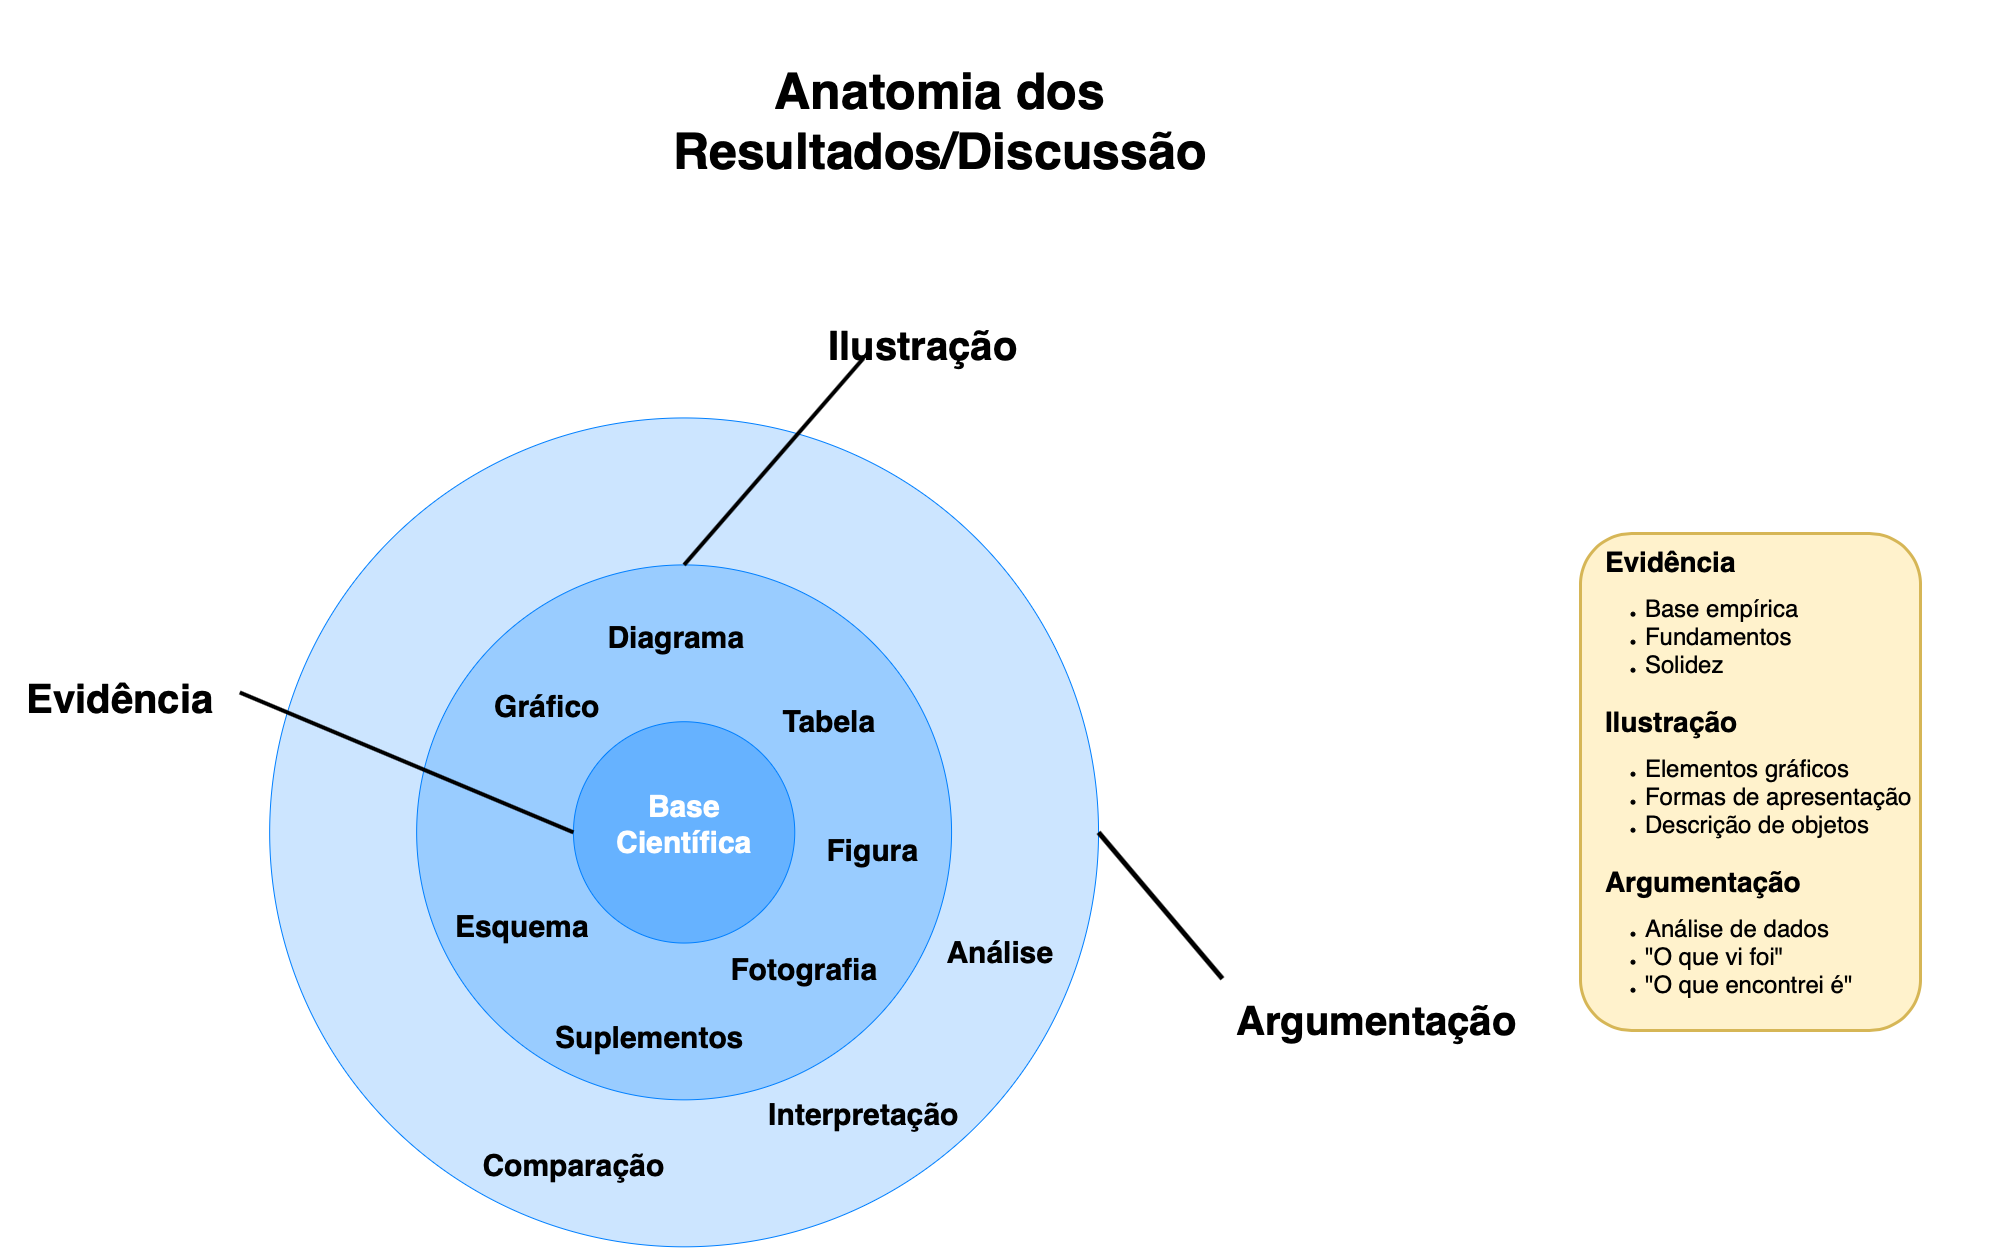
\includegraphics[scale=0.14]{figs/07/resultados-discussao}
\caption{Baseado em (Zucolloto, 2011) e (Volpato, 2017). Fonte: Autor.}
\end{figure}
\end{frame}

\begin{frame}{Dimensões}
\begin{itemize}
\item \textbf{Evidência}: use uma base empírica forte e confiável para construir 
\item \textbf{Descrição}: use figuras, tabelas, desenhos e esquemas para embelezar
\item \textbf{Argumentação}: use texto, palavras e argumentos para sustentar
\end{itemize}
\end{frame}

\begin{frame}{Formas de apresentação}
\begin{itemize}
\item Figura: gráficos, fotografias, desenhos, esquemas
\item Tabela: números, palavras, desenhos
\item Texto: números, palavras
\item Material suplementar: arquivos de som e vídeo, interativos 
\end{itemize}
\end{frame}

\subsection{Apresentação da informação}

\begin{frame}{Ênfase das formas}
\begin{itemize}
\item Figuras (muito evidente; atrai muita atenção)
\item Tabelas (evidente; atrai atenção)
\item Texto (pouco evidente; atrai pouca atenção)
\end{itemize}
\end{frame}

\begin{frame}{Critério da forma}
\begin{figure}
\centering
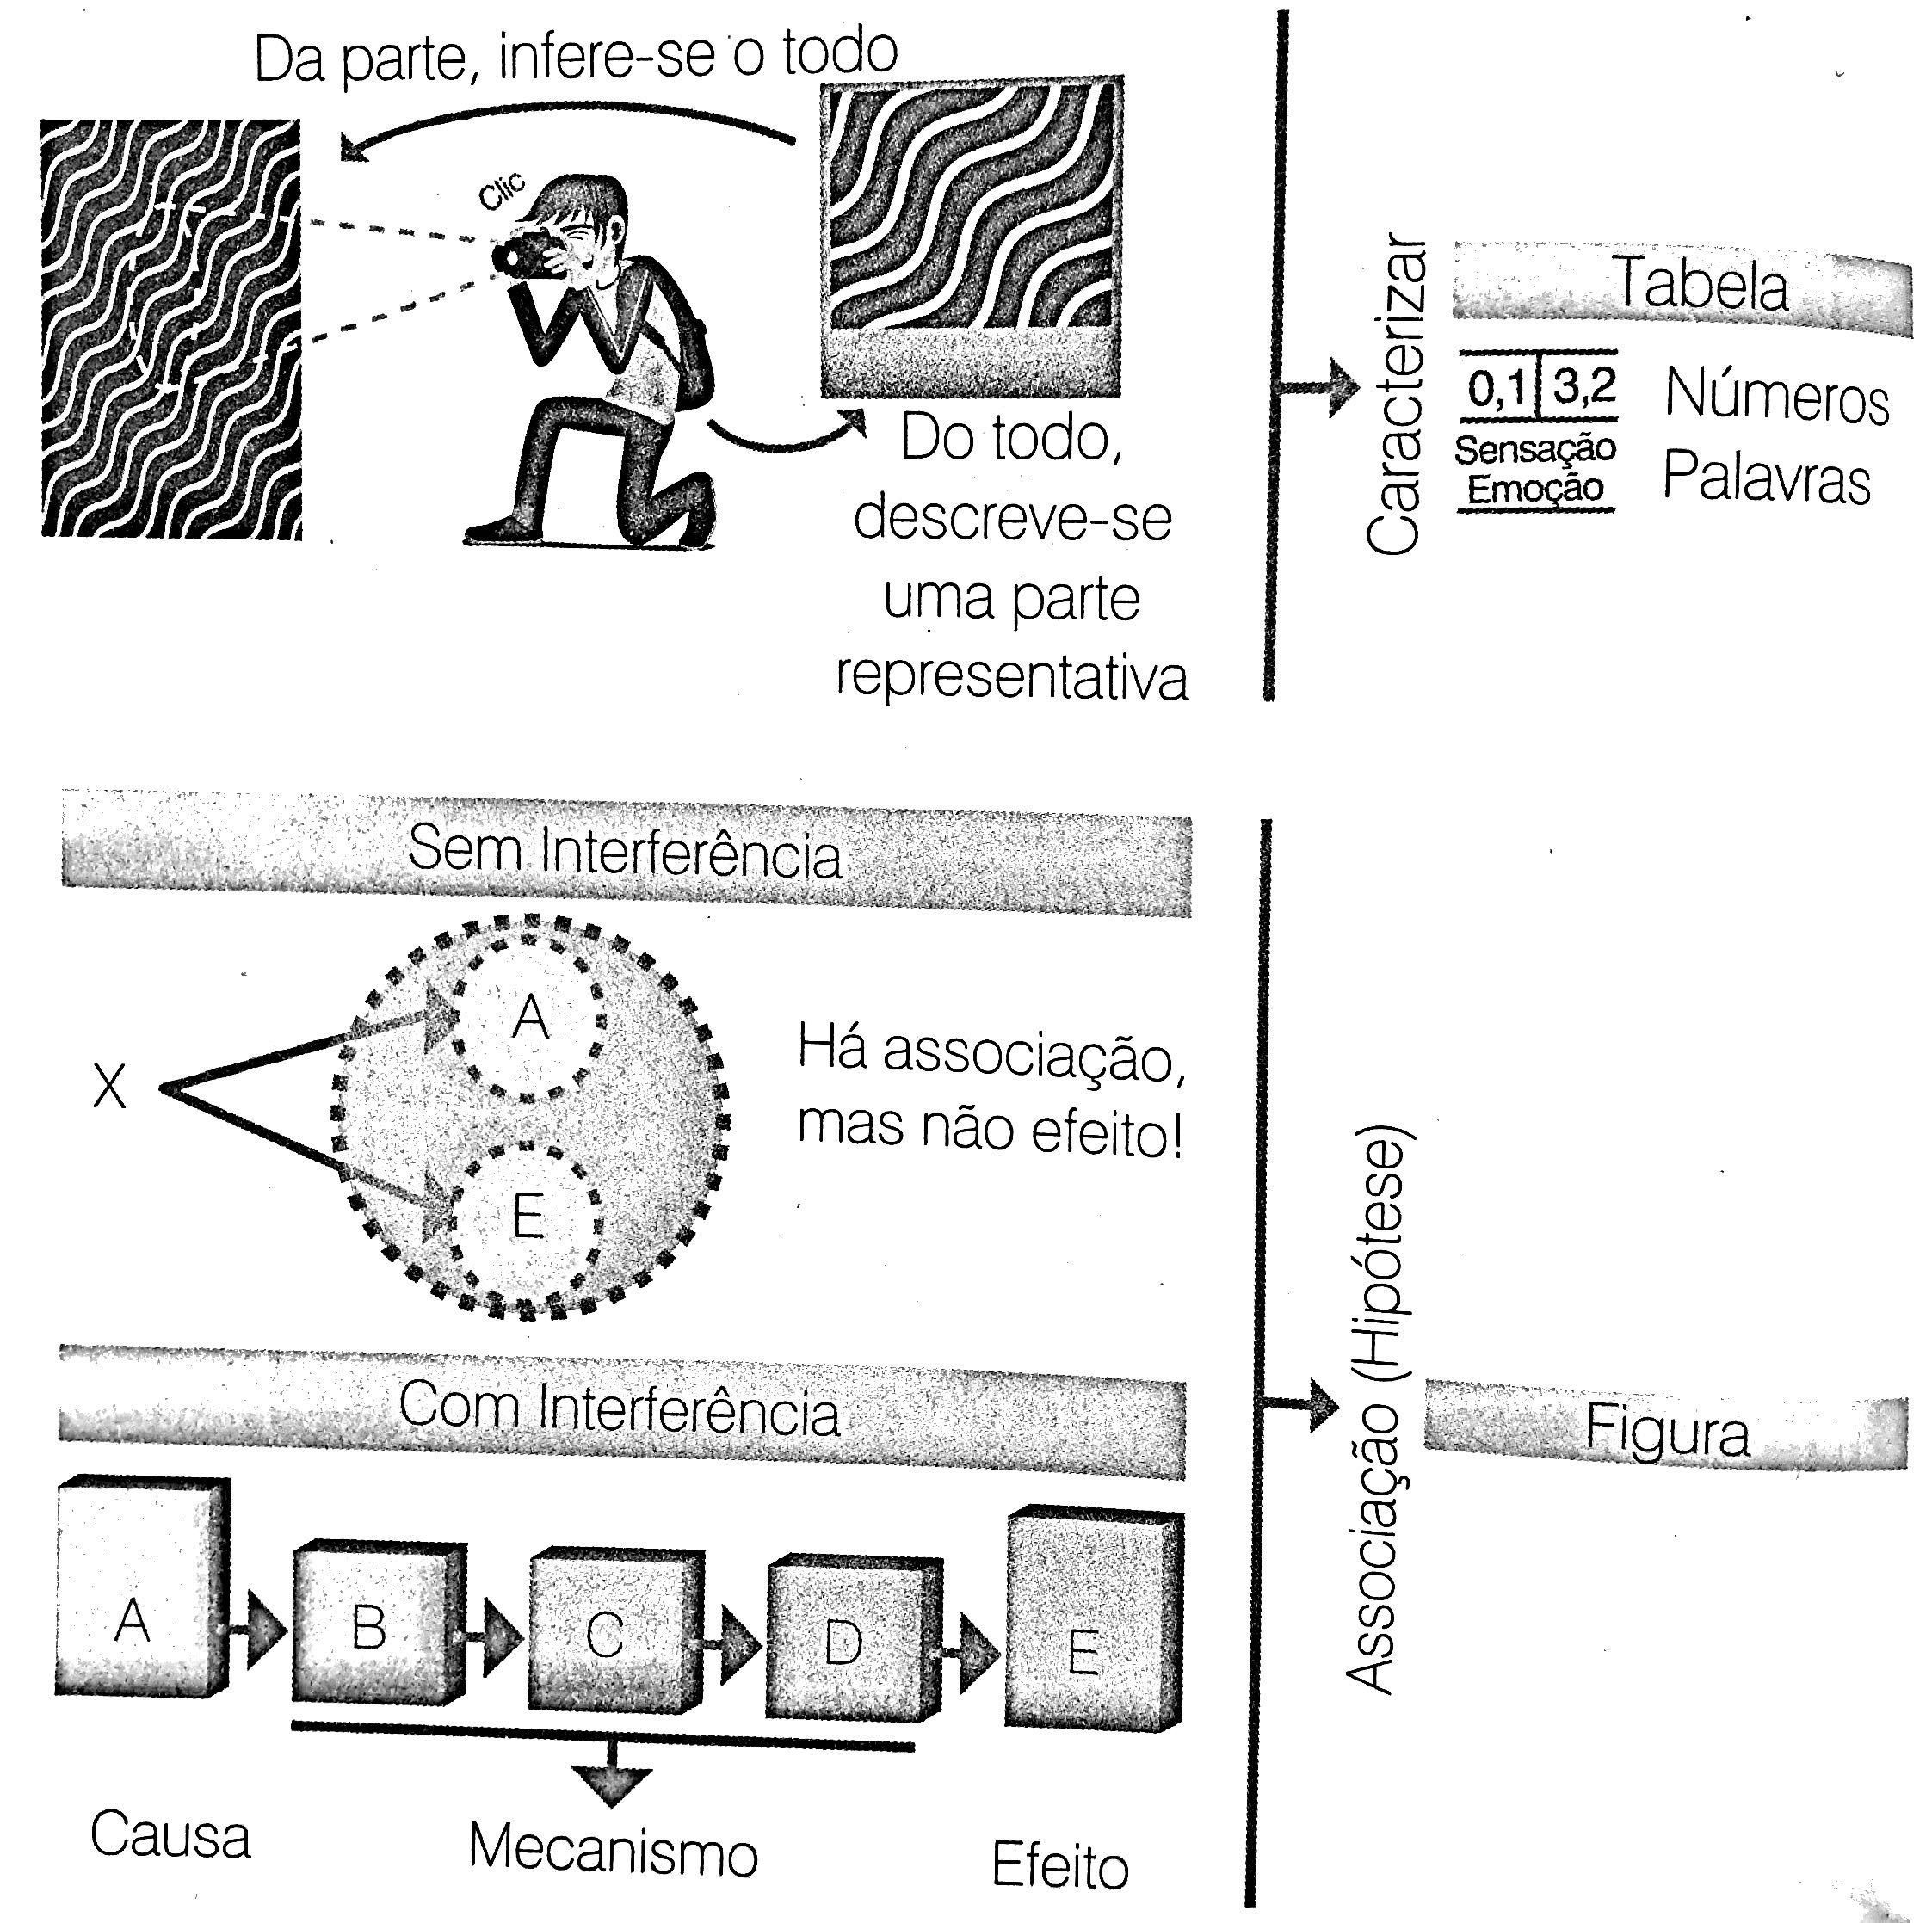
\includegraphics[scale=0.08]{figs/07/criterio-forma}
\caption{Critério lógico: formato. Fonte: Volpato (2017).}
\end{figure}
\end{frame}

\begin{frame}{cont.}
\begin{itemize}
\item Pesquisa de caracterização (enxergar valores quantitativa e qualitativamente): tabela 
\item Teste de hipóteses (enxergar relações de causa/efeito): figura
\end{itemize}
\end{frame}

\begin{frame}{Critério da ênfase}
\begin{itemize}
\item Esclarecer o que viu! 
\item O que traz indícios para maior ou menor ênfase? 
\item X é uma variável muito frequente, presente, relevante, destacada? Fale mais sobre ela!
\item Y é uma variável que quase não apareceu na história? Fale uma vez só sobre ela!\\
\item Necessário usar figura? Tabela? Texto resolve? Se sim, pronto. 
\end{itemize}
\end{frame}

\begin{frame}{Critério do contexto}
\begin{figure}
\centering
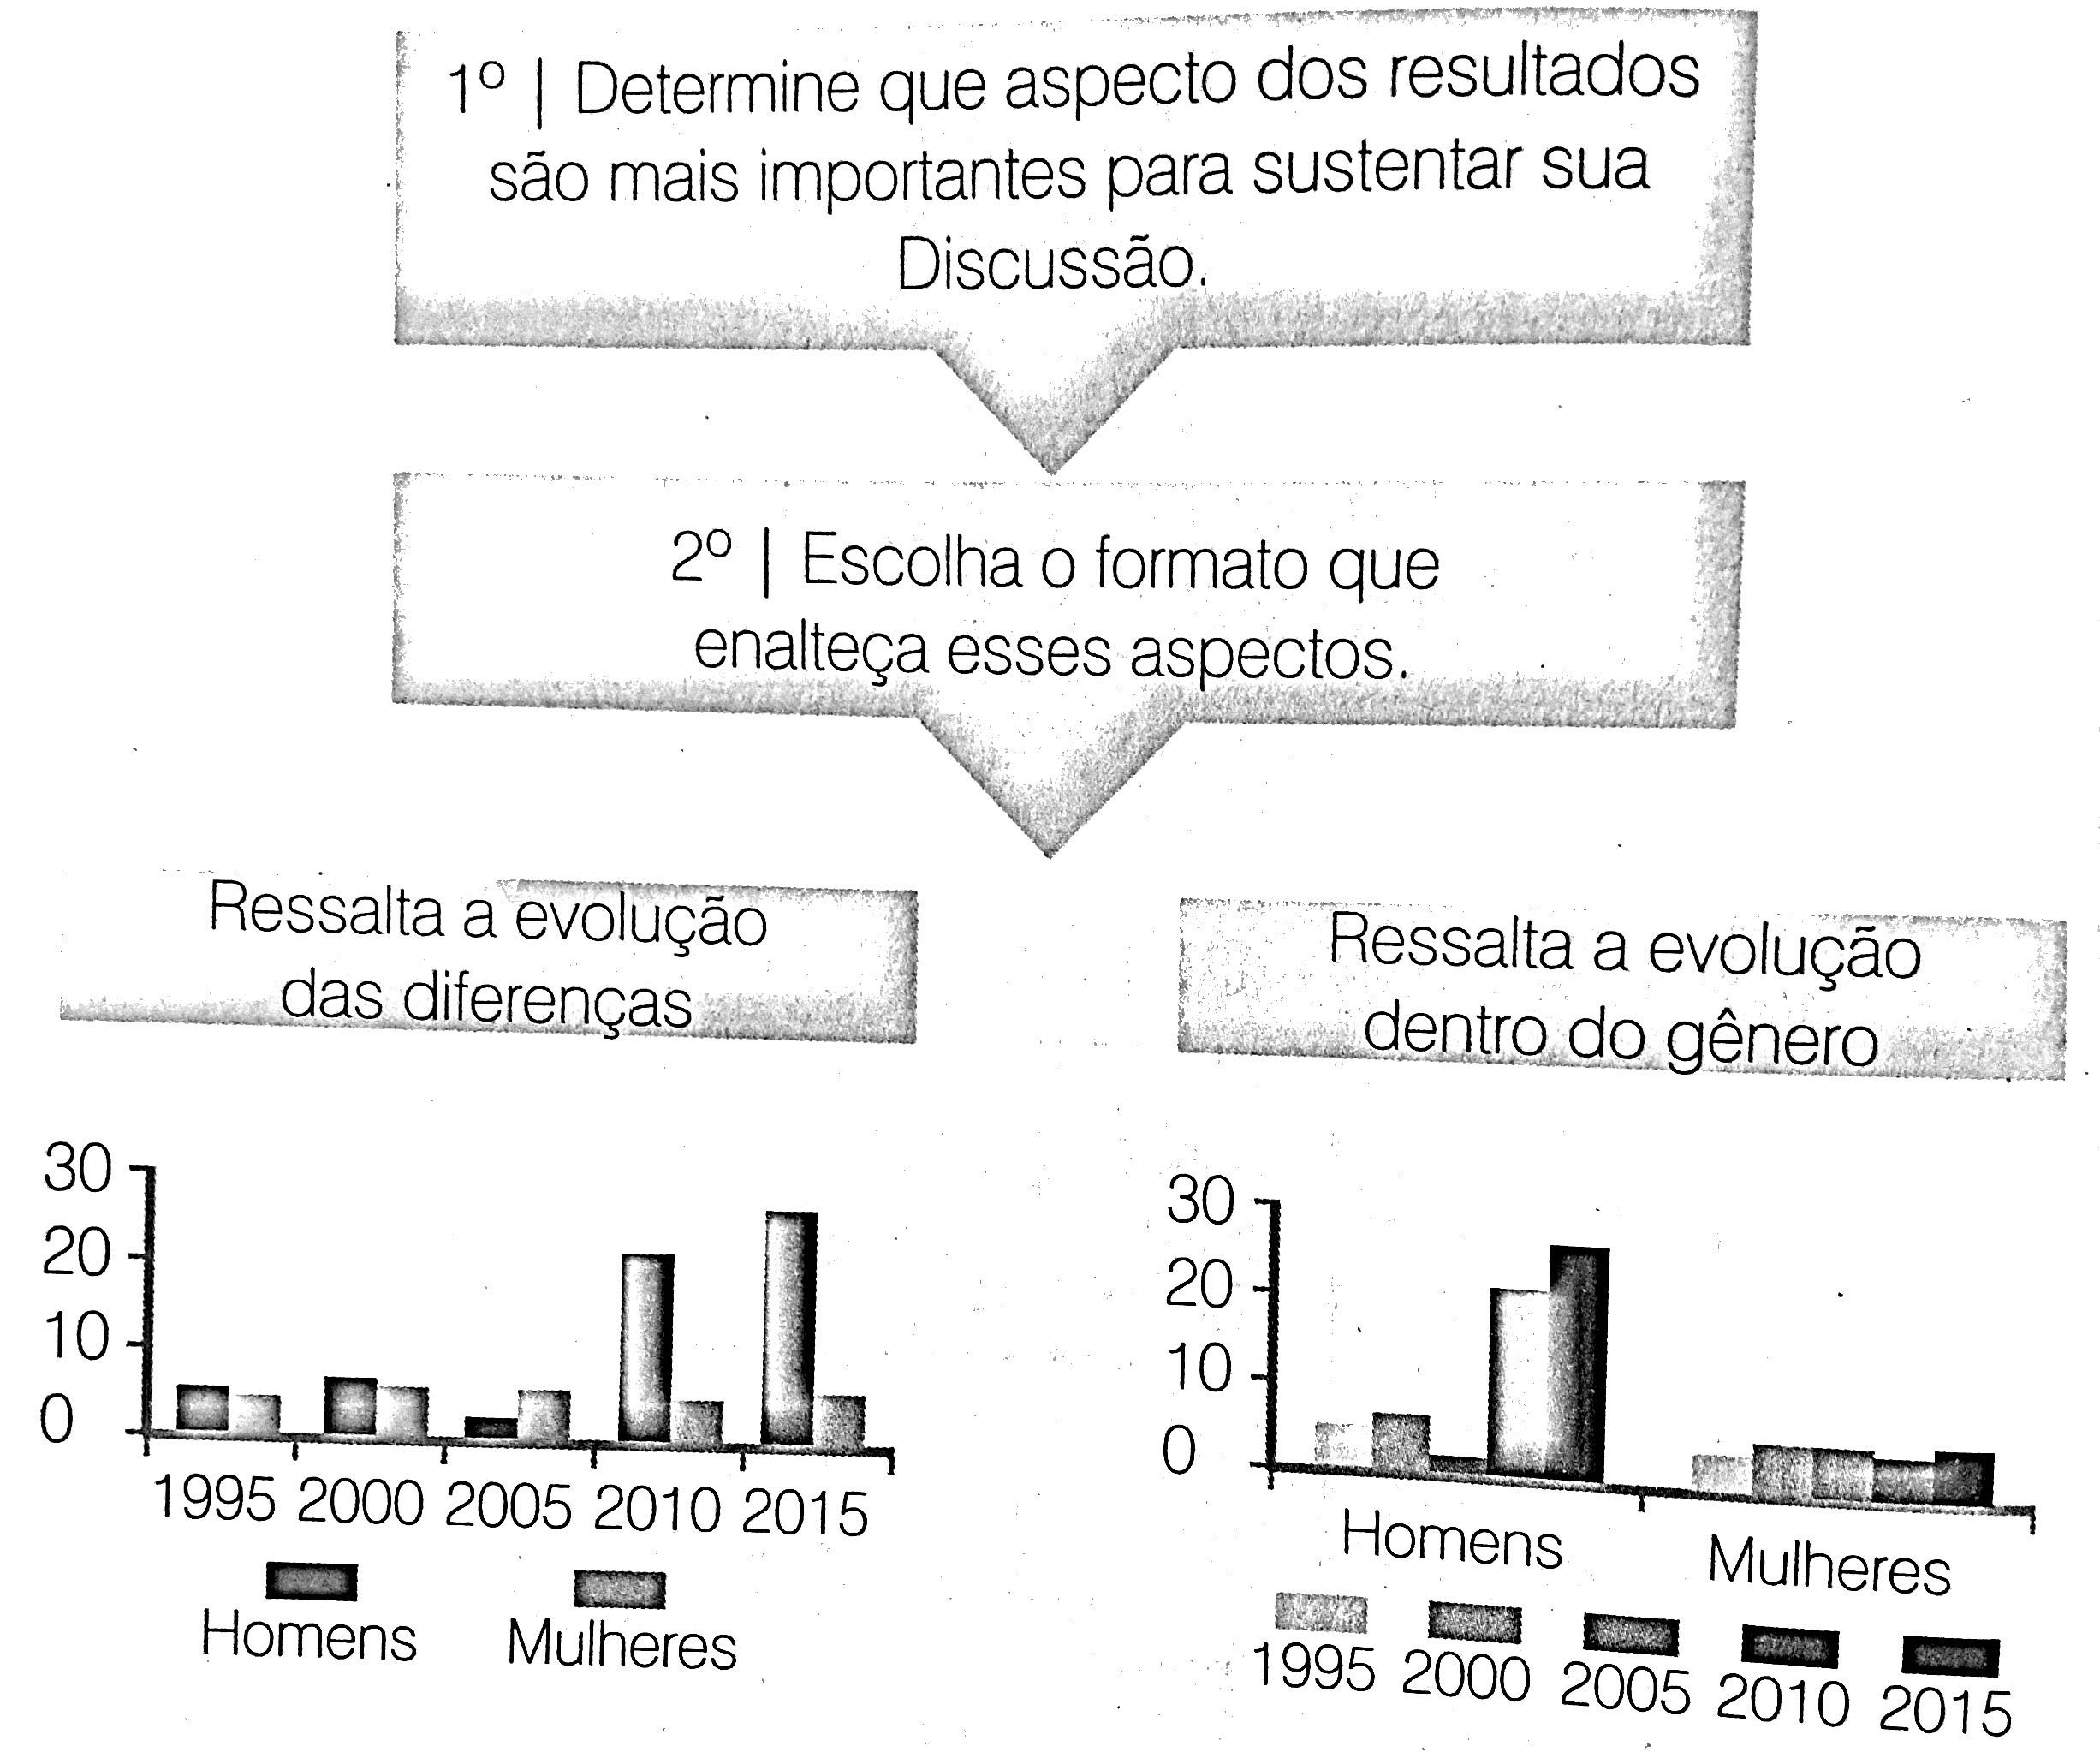
\includegraphics[scale=0.08]{figs/07/criterio-contexto}
\caption{Critério lógico: contexto. Fonte: Volpato (2017).}
\end{figure}
\end{frame}

\begin{frame}{cont.}
\begin{itemize}
\item Tabelas e figuras têm mútliplas formas de apresentação
\item Use o critério anterior para definir os papéis 
\item Ex.: figura da esquerda enfatiza comparação entre H/M com evolução temporal
\item Ex.: figura da direita enfatiza a evolução temporal de H/M dentro de cada gênero 
\end{itemize}
\end{frame}

\begin{frame}{Legendas}
\begin{itemize}
\item Inclua detalhes nas legendas de tabelas e figuras  
\item Especificações suficientes para perfeito entendimento
\item Descreva e faça associações 
\item Não repita nomes de variáveis, interprete 
\end{itemize}
\end{frame}

\begin{frame}{Interpretação de dados}
\begin{itemize}
\item Não jogue o leitor na brasa!
\item No texto, faça referências a tabelas, figuras e dados ``guiando o leitor''
\item Faça a ``leitura'' dos dados e facilite a compreensão do leitor
\item Ex.: ``Os dados de aumento volumétrico com a pressão estão na Tabela X'' (ruim)
\item Ex.: ``O volume cresce a uma taxa de 20\% quando a pressão interna mantém-se em 1.3 bar (Tabela X)''
\end{itemize}
\end{frame}

\subsection{Características da ``boa discussão''}

\begin{frame}{Propósito da discussão}
\begin{block}{Relações factuais}
A discussão serve para destacar relações entre os fatos observados
\end{block}
\end{frame}

\begin{frame}{O que observar?}
\begin{itemize}
\item Atenha-se ao que os resultados mostraram 
\item Discuta, não recapitule! 
\item Aponte exceções, faltas de correlação ou pontos inconclusivos
\item Mostre concordâncias/contrastes entre resultados e interpretações 
\item Fale das implicações teóricas dos resultados sem timidez 
\item Conecte evidências para cada conclusão
\end{itemize}
\end{frame}

\section{Como escrever a Conclusão}

\begin{frame}{O que fazer?}
\begin{itemize}
\item Resuma os principais resultados 
\item Seja breve e coerente com a discussão
\item Seja moderado com ``trabalhos futuros'' e promessas
\item Inclua pontos de vista sobre como o trabalho pode oportunizar pesquisas
\end{itemize}
\end{frame}


\section{Como registrar Agradecimentos}

\begin{frame}{A seção}
\begin{itemize}
\item \emph{Acknowledgments} é uma seção destinada a ``notas de reconhecimento''
\item Seu propósito é agradecer por contribuições e exercitar a cortesia
\item Não há nada de científico aqui, mas também não há romance... 
\end{itemize}
\end{frame}

\begin{frame}{Ingredientes}
\begin{itemize}
\item Agradeça a pessoas por auxilío técnico (laboratorial, uso de equipamentos, organização de materiais, auxílio computacional, etc.) 
\item Agradeça instituições por fomentos à pesquisa que gerou o artigo (auxílios, bolsas, financiamento)
\item Eventualmente, agradeça os revisores por sugestões valiosas
\end{itemize}
\end{frame}

\subsection{Bons exemplos de agradecimentos}

%%
\begin{frame}
\begin{block}{Pessoa}
\emph{I would like to thank Mr. Enius Atis for technical assistance with facility, Ela Doris for her kind help with the experiments and Denis Graus for computational support.}
\end{block}

\begin{block}{Pessoa}
\emph{A.L.P. is indebted to Dr. Alefis Onexis for making the datasets A23c and B44f available to this research.}
\end{block}
\end{frame}

%%
\begin{frame}
\begin{block}{Instituição}
\emph{The authors thank to Manopano Co. for funding this research.}
\end{block}

\begin{block}{Instituição}
\emph{J.P.G thanks to the Brazilian National Council for Scientific and Technological Development (CNPq) for her scholarship.}
\end{block}
\end{frame}

%%
\begin{frame}
\begin{block}{Instituição}
\emph{Amy Plenis thanks to SCNF for his fellowship. Deo Solis would like to thank Copy and Paste Brazil for the financial support (R{\&}D grant no. 201909-07).}
\end{block}

\begin{block}{Revisor}
\emph{The authors acknowledge the reviewers for their invaluable comments.}
\end{block}
\end{frame}

\subsubsection{O que não dizer nos agradecimentos}

\begin{frame}{Alguns maus exemplos}
\begin{block}{Pessoa}
\emph{I wish to thank Do Go for this... that...}  
\end{block}

\begin{block}{Instituição}
\emph{I wish to thank CNPq for my scholarship.}  
\end{block}

\begin{block}{Revisor}
\emph{I want to thank the reviewers for their incredible comments which helped a lot this paper to be improved.}  
\end{block}
\end{frame}

%
\section{Exercício in-class}
%
%%%
\begin{frame}{Tarefas}
\begin{enumerate}
\item Formem 5 grupos e selecionem 1 líder por grupo
\item Cada grupo deverá analisar a seção de resultados/discussões do artigo a seguir
\item Cada grupo responderá o máximo do questionário a seguir
\item Cada líder anotará as respostas de seu grupo em uma lista
\item No final, debateremos as análises apresentadas
\end{enumerate}
\end{frame}

\begin{frame}{Artigo para análise} 
\begin{itemize}
\item 01-Bonati2019-JMPS, \url{https://doi.org/10.1016/j.jmps.2018.08.022}
\end{itemize}
\end{frame}

%%
\begin{frame}{Questionário}
\begin{enumerate}
\item Qual(is) forma(s) de apresentação de dados são utilizadas? Qual é predominante? 
\item É possível compreender a mensagem das figuras apenas lendo suas legendas? 
\item Excertos onde ocorrem relações factuais explícitas são detectáveis? Exemplifique.
\item O(s) autor(es) comentam algo sobre exceções, limitações ou implicações dos resultados? Exemplifique. 
\item Em algum momento no texto, mostram-se contrastes ou comparações entre resultados e interpretações? Dê exemplos.
\end{enumerate}
\end{frame}

%% === REFS
\begin{frame}[allowframebreaks]
\frametitle{Referências}
\begin{thebibliography}{9}
\setbeamertemplate{bibliography item}[book]
%
\bibitem{volpato2017}Volpato, G.L. \textit{Método Lógico para Redação Científica}. 2a. ed., Best Writing, 2017.
%
\bibitem{zuco2011}Zucolotto, V. \textit{Workshop de Capacitação em Escrita Científica}, Disponível em: \url{http://www.escritacientifica.sc.usp.br/escrita/cursos-escrita/}
%
\bibitem{day1993} Day, R. A., \textit{How to write and publish a scientific paper}, Cambridge University Press, 1995.
\end{thebibliography}
\end{frame}